\chapter{What does entanglement have to do with computer science ?}
\section{Introduction}
L'idée est d'utiliser les qbits pour avoir des algorithmes plus efficace, mais ceux-ci
sont fragiles et se détruisent vite. A cause de la \textit{décohérence} qui est une source
forte d'erreurs, on perd rapidement toutes les belles propriétés quantiques comme la superposition. \\

Au début, à cause de la décohérence, tout était théorique. Mais après est venu l'idée de 
prolonger l'idée des codes correcteurs d'erreur au monde quantique. A cause du \textit{théorème
de non-clonage quantique} (cours 3) qui dit qu'un qbit ne peut pas être parfaitement cloné, on
pourrait croire qu'on ne peut pas faire des codes correcteurs d'erreurs. Nous montrerons cependant
que nous pouvons.

\subsection{Correction d'erreur classique}
	\begin{wrapfigure}[5]{r}{4cm}
	\vspace{-5mm}
	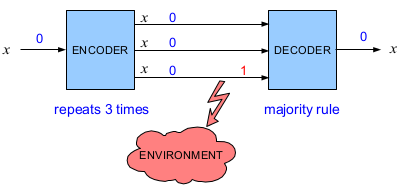
\includegraphics[scale=0.3]{ch2/image1.png}
	\captionof{figure}{ }
	\end{wrapfigure}
Il s'agit du cas classique et trivial, c'est le codage répétitif (on introduit de la redondance). Le même
bit est dupliqué trois fois et on l'envoie. Il peut y avoir des erreurs à cause de l'environnement que
l'on peut corriger via cette redondance. Mais en quantique, on ne peut pas faire ça.

\subsection{Correction d'erreur quantique}
	\begin{wrapfigure}[7]{r}{7cm}
	\vspace{-5mm}
	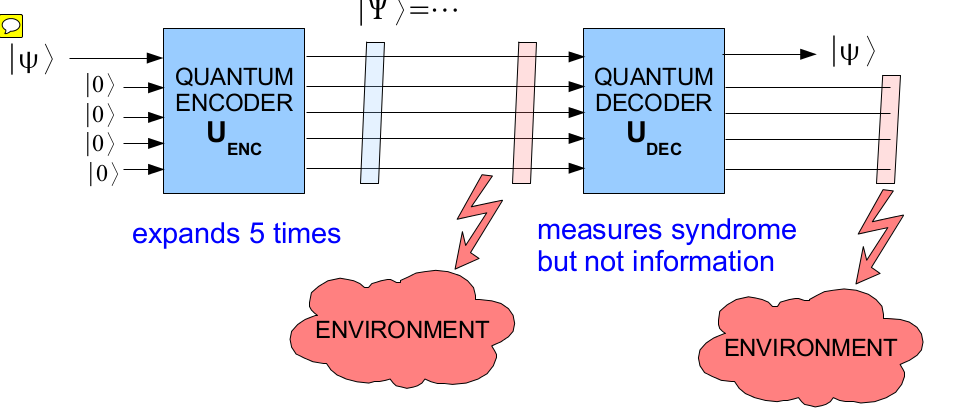
\includegraphics[scale=0.2]{ch2/image2.png}
	\captionof{figure}{ }
	\end{wrapfigure}
Soit un qbit $\ket\psi = \alpha\ket0+\beta\ket1$. On l'envoie dans un encodeur quantique $U_{ENC}$ 
avec une superposition quantique, n'importe laquelle (ici $n=4$). Nous allons faire une opération 
telle que les cinq états de qbits sont \textbf{intriqués} (on ne peut pas les décomposer dans un état pur
de chaque qbit) : ils définissent un état pur pour les 5 qbits \textbf{ensemble}.\\

Il y a des interaction avec l'environnement et, imaginons, le 5$^e$ qbit est touché. Vient le 
décodage avec $U_{DEC}$ ou le \textit{syndrome} est séparer de l'\textit{information}. Le syndrome
informe qu'il y a eu une erreur sur le 5$^e$ qbit (par exemple, il a flip). Durant le décodage, on 
sépare donc le syndrome (quatre derniers qbits) et l'information (le premier).\\

Si on mesure les quatre bits à la fin, on verra le sydrome et ce qui est arrivé au qbit. Mais 
nous n'avons pas besoin de cette information : ce qui importe, c'est d'avoir $\ket\psi$ à la fin. 
C'est le rôle du décodeur, mais nous n'explicitons pas comment il procède. Nous ne voulons pas
mesurer $\ket\psi$ car la mesure détruit l'information. Le truc, c'est qu'une erreur qui affecte
un des cinq qbits peut être restaurée car quand l'environnement jour son rôle, le qbit est intriqué.
L'idée est donc bien d'encoder un qbit dans cinq qbit et que celui-ci puisse survivre de l'erreur
sur un des cinq qbits (interaction avec l'environnement) via l'opération de décodage. \\

\textbf{This course}\\
\textit{Que vient faire l'intrication quantique dans la science informatique ? } Application : 
\textit{distributed computing problem}.




\section{What does entanglement have to do with computer science ?}
Nous allosn réinterpréter un paradoxe quantique en langage de l'information. Nous allons ensuite
l'appliquer sur un problème académique puis sur un problème "réel". 

\subsection{Problème académique}
	\begin{wrapfigure}[11]{l}{6.5cm}
	\vspace{-5mm}
	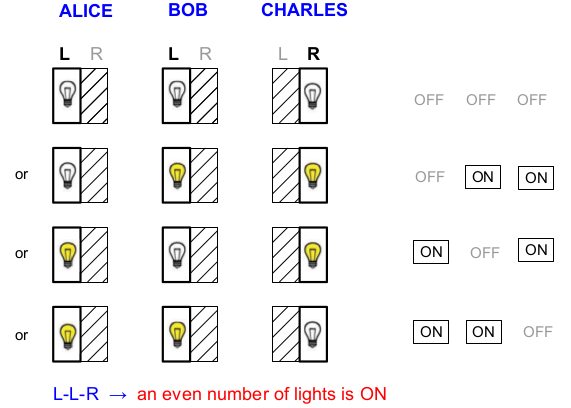
\includegraphics[scale=0.3]{ch2/image5}
	\captionof{figure}{ }
	\end{wrapfigure}
\textbf{A}lice, \textbf{B}ob et \textbf{C}harles achètent tous les trois une \textit{magic box} 
dans une \textit{magasin quantique} et ils s'en vont tous les trois dans des pays différents. Ensuite,
chacun ouvre la moitié de sa boite (partie gauche $L$ et droite $R$) pour y voir une ampoule
allumée (\textit{on}) ou éteinte (\textit{off}).\\

Alice et Bob décident tous deux d'ouvrir la partie gauche tandis que Charles ouvre la partie de 
droite : configuration $LLR$. Il y a plusieurs possibilité (On/Off), mais dans tous les cas, un
nombre \textbf{pair} de lumière est \textit{on}. Dans la configuration $RLL$ (permutation cyclique),
le constat est le même : un nombre \textbf{pair} de lumière est \textit{on}.\\

Dans les configuration $LLR, RLL$ et $LRL$, nous devons avoir un nombre pair de \textit{on}. Nous
allons essayer de décrire mathématiquement ce que nous avons observés en définissant un bit de la
sorte
\begin{equation}
\left\{\begin{array}{ll}
On &\equiv +1\\
Off&\equiv -1
\end{array}\right.\qquad\qquad (-1)^{0,1}
\end{equation}
Notre situation correspond donc à
\begin{equation}
\begin{array}{lll}
LLR &\to A_L\times B_L\times C_R &=+1\\
RLL &\to A_R\times B_L\times C_L &=+1\\
LRL &\to A_L\times B_R\times C_L &=+1
\end{array}
\end{equation}
Alice, Bob et Charles sont spatialement séparés : aucun d'eux ne sait si les deux autres ont 
regardés la partie gauche ou droite de leur boîte. Juste par causalité, Alice ne peut pas 
avoir des informations sur Bob et Charles : quand elle ouvre, elle est ignorante. Nous pouvons
ainsi faire l'hypothèse que les variables $L$ et $R$ \textbf{existent} : Alice n'a peut-être
pas regardé $A_R$, mais la variable existe (et c'est le cas pour les six variables).\\

Nous pouvons faire une prédiction grâce à ce modèle simple si l'on effectue la multiplication
colonne par colonne. En effet, $A_L*A_L*A_R = A_L^2*A_R=A_R$, on en tire donc
\begin{equation}
RRR\quad\to A_R\times B_R\times C_R = +1
\end{equation}
Le nombre de lumière allumée devrait être \textbf{pair} dans la configuration $RRR$. Malheureusement,
l'expérience nous montre que c'est un nombre \textbf{impair}\footnote{C'est pas une explication ici,
une observation}. Il y a donc quelque chose de faux dans notre modèle.\\

Récapitulons. Nous avons six variables
\begin{equation}
A_L,A_R, B_L,B_R,C_L,C_R \in \{+1,-1\}
\end{equation}
\begin{description}
\item[Prédiction] $A_R\times B_R\times C_R = +1$. En \textbf{supposant} que ces variables 
existent simultanément. 
\item[Observation] $A_R\times B_R\times C_R = -1$. En réalisant que ces boîtes magiques
contiennent des \textbf{qbits}.
\end{description}
Supposer que les six variables existent en même temps ne peut être que faux. Comment s'en sortir?

\subsection{Quantum miracle}
La physique classique ne parvient pas à expliquer l'observation, la solution sera un état intriqué. On
assigne à $A$ le bit 1, $B$ le second et $C$ le troisième mais nous les décrivons \textit{ensemble}
\begin{equation}
\ket\Psi = \frac{1}{\sqrt{2}}\left\{\ket{0,0,0}_{A,B,C}-\ket{1,1,1}_{A,B,C}\right\}\qquad
\text{"GHZ"}
\end{equation}
Il s'agit de la superposition de deux états, mais intriqués. $A,B$ et $C$ ne peuvent pas être
dans un état pur, on doit les décrire ensemble : on ne peut pas les exprimer comme un produit.\\

Choisissons la convention (base) suivante
\begin{equation}
\ket0\equiv\left(\begin{array}{c}
1\\
0
\end{array}\right)\qquad\qquad\ket1\equiv\left(\begin{array}{c}
0\\
1
\end{array}\right)
\end{equation}
Il s'agit de deux vecteurs d'un espace 2D. Une mesure doit être associée à un observable. On 
va utiliser les matrices de \textsc{Pauli} qui correspondent à la mesure du spin. Ainsi, si 
le qbit est un spin $1/2$, $\sigma_x$ mesure la composante de spin dans l'axe $x$. Les trois
matrices de Pauli sont les suivantes
\begin{equation}
\begin{array}{ccc}
\sigma_x = \left(\begin{array}{cc}
0&1\\
1&0
\end{array}\right) &\qquad \sigma_y = \left(\begin{array}{cc}
0&-i\\
i&0
\end{array}\right) &\qquad \sigma_z = \left(\begin{array}{cc}
1&0\\
0&-1
\end{array}\right)\\
\text{BIT FLIP} &\qquad \leftarrow \text{BOTH}\rightarrow &\qquad \text{SIGN FLIP}\\
\left\{\begin{array}{ll}
\sigma_x\ket0 &= \ket 1\\
\sigma_x\ket1 &= \ket 0
\end{array}\right. &\qquad\left\{\begin{array}{ll}
\sigma_y\ket0 &= i\ket 1\\
\sigma_y\ket1 &= -i\ket 0
\end{array}\right.&\qquad\left\{\begin{array}{ll}
\sigma_z\ket0 &= \ket 0\\
\sigma_z\ket1 &= -\ket 1
\end{array}\right.
\end{array}
\end{equation}
On peut ainsi voir $\sigma_x$ comme un \textit{bit flip} : si on l'applique sur $\ket0$ on obtient
un $\ket 1$ et inversement. Ça correspond à une porte \textit{NOT}. La matrice $\sigma_z$ correspond
au \textit{sign flip} : $\ket 0$ reste lui-même mais $\ket1$ change de signe. Les valeurs propres
des matrices de \textsc{Pauli} sont les suivantes
\begin{equation}
\left\{+1,-1\right\} \equiv \{OFF,ON\}
\end{equation}
Supposons maintenant que l'action \textit{ouvrir à gauche} $L$ corresponde à mesurer $\sigma_y$ et 
$R$ corresponde à $\sigma_x$. Traduisons notre précédent système en langage quantique
\begin{equation}
\begin{array}{lll}
LLR&\to \sigma_y\otimes\sigma_y\otimes \sigma_x\ket\Psi &=\ket\Psi\\
RLL&\to \sigma_x\otimes\sigma_y\otimes \sigma_y\ket\Psi &=\ket\Psi\\
LRL&\to \sigma_y\otimes\sigma_x\otimes \sigma_y\ket\Psi &=\ket\Psi
\end{array}
\end{equation}
avec $\ket\Psi = \frac{1}{\sqrt{2}}\left\{\ket{0,0,0}_{A,B,C}-\ket{1,1,1}_{A,B,C}\right\}$ et chaque
matrice de Pauli porte sur un qbit différent. On retrouve bien à chaque fois $\ket\Psi$, ce qui
signifie que le nombre de lumière allumée est \textbf{pair}. On peut dire que $\ket\Psi$ est un
état propre commun du produit de ces trois observables avec comme valeur propre $+1$.\\

Une propriété importante des matrices de \textsc{Pauli} est leur anti-commutation : il faut placer
un "-" lorsqu'on change l'ordre. C'est ce qui va produire le \textit{miracle quantique}.
\begin{equation}
\{\sigma_x,\sigma_y\} \equiv \sigma_x\sigma_y+\sigma_y\sigma_x=0
\end{equation}
Essayons de refaire notre prédiction. Nous allons refaire le produit mais cette fois-ci il 
s'agit d'un produit matriciel qui ne commute pas ! On va faire l'opérateur de la première lignes
$\times$ celui de la seconde $\times$ celui de la troisième. Ceci est équivalent à faire
le produit de la première colonne $\times$ celui de la seconde $\times$ celui de la troisième. Pour
la première colonne, nous avons
\begin{equation}
\sigma_y\sigma_x\sigma_y = -\sigma_y\sigma_y\sigma_x = -\sigma_y
\end{equation}
car $\sigma_y^2=\hat{1}$ (le \textit{double flip}, c'est l'identité). En faisant de même pour
les deux autres colonnes (ou chaque fois nous avons directement un $\sigma_y^2$)
\begin{equation}
RRR\quad\to \sigma_x\otimes\sigma_x\otimes\sigma_x\ket\Psi = -\ket\Psi
\end{equation}
C'est le \textit{miracle quantique}, le nombre de lumière allumée est \textbf{impair} ! Ceci 
colle aux observations. Le $\ket\Psi$ est un étant propre de ce quatrième produit d'observable, mais
de valeur propre $-1$.


\subsubsection{Solution au miracle quantique}
	\begin{wrapfigure}[9]{l}{7cm}
	\vspace{-5mm}
	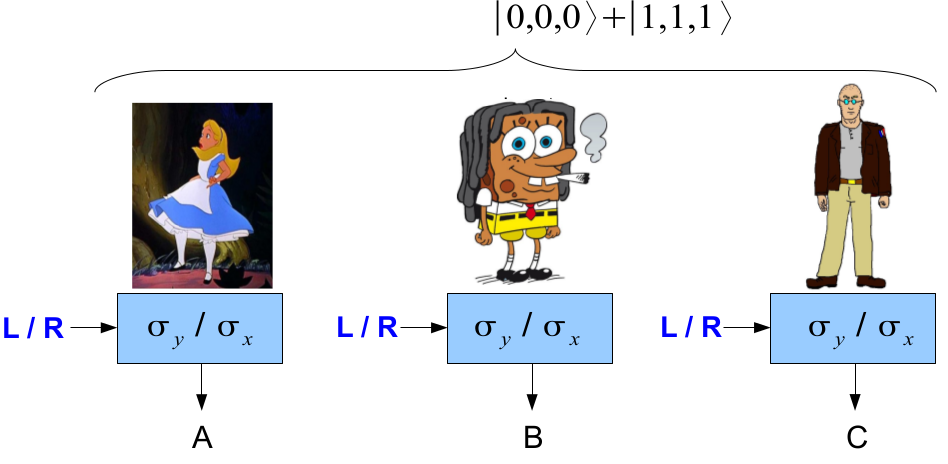
\includegraphics[scale=0.2]{ch2/image4.png}
	\captionof{figure}{ }
	\end{wrapfigure}
On peut prendre un des états GHZ préparé et on met un qbit dans chacune des boîtes. En fonction de
ce qu'ils ouvrent, ils utilisent $\sigma_x$ ou $\sigma_y$. Tout est réglé car les deux possibilités
($L$ ou $R$) correspondent aux deux mesures. On dit que $\sigma_x$ et $\sigma_y$ sont 
\textbf{incompatibles} : on ne peut pas les définir ensemble car ils anticommutent. Si l'on a un
spin $1/2$, on ne peut pas lui associer un $\sigma_x$ et un $\sigma_y$ en même temps. On peut en
connaître un, mais pas le second. En mécanique quantique, on ne peut pas donner une valeurs 
aux "deux ensembles". Alice a un qbit : on ne peut pas avoir à la fois précisément la valeur donnée
par $\sigma_y$ et celle par $\sigma_x$ car cela violerait le principe d'incertitude. 

\subsection{Problème réel : distributed computing}
Comment est-ce que ceci peut être utilisé dans un contexte informationnel? Supposons que nous avons
à nouveau trois parties $A,B$ et $C$ et que chacune d'elles reçoit une chaîne de bits
\begin{equation}
x=\underbrace{010110\dots}_{n\ bits}\to A,\qquad\qquad
y=\underbrace{111001\dots}_{n\ bits}\to B,\qquad\qquad
z=\underbrace{010000\dots}_{n\ bits}\to C
\end{equation}
Alice aimerait bien calculer l'addition modulo 2 suivante
\begin{equation}
f(x,y,z) = x_1y_1z_1\oplus x_2y_2z_2\oplus\dots \oplus x_ny_nz_n
\end{equation}
sachant que $x\oplus y\oplus z=(x_1\oplus y_1\oplus z_1,x_2\oplus y_2\oplus z_2,\dots,x_n\oplus y_n\oplus z_n) = (1,1,\dots,1)$. On veut calculer
$f(x,y,z)$ en minimisant au maximum la communication, sinon $B$ n'aura qu'a tout envoyer à $A$ et 
ce serait fini. \\

C'est le \textit{distributed computing problem} : comment calculer $f(x,y,z)$ qui a des entrées
distribuées dans les trois parties en gardant la communication entre les parties la plus faible
que possible ? Il existe des algorithmes classiques dont la complexité de cet algorithme est 
de $C=3$bits\footnote{Par exemple, $C$ envoie 1 bit à $A$ qui en envoie 2 à $B$.}


\subsubsection{Comment faire mieux?}
	\begin{wrapfigure}[6]{l}{7cm}
	\vspace{-5mm}
	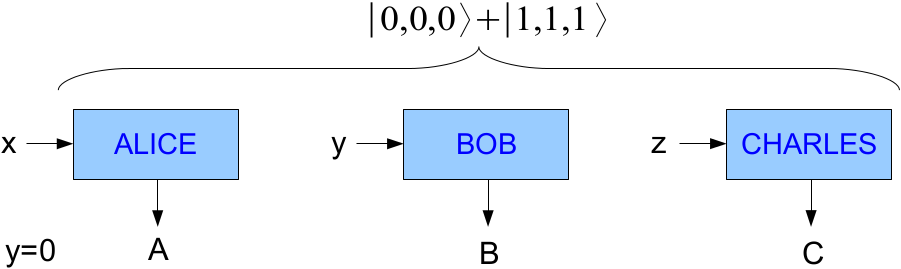
\includegraphics[scale=0.2]{ch2/image3.png}
	\captionof{figure}{ }
	\end{wrapfigure}
On prépare un état GHZ global pour $A,B$ et $C$ à qui on donne un chaîne de qbit, comme précédemment
(resp. $x,y$ et $z$). On regarde chacun des bits de la chaîne, un à un. Si la variable d'entrée est 
nulle ($x=0,y=0$ ou $z=0$) cela correspond à l'action $L$ (définie par $\sigma_y$). Sinon, c'est $R$
 (définie par $\sigma_x$). Nous avons comme précédemment\footnote{Comment?! Pourquoi des addition 
 maintenant?! Quel est l'avantage d'être quantique alors?}
\begin{equation}
\begin{array}{lll}
LLR&\to A\oplus B\oplus C &=0\\
RLL&\to A\oplus B\oplus C &=0\\
LRL&\to A\oplus B\oplus C &=0\\
RRR&\to A\oplus B\oplus C &=1
\end{array}
\end{equation}
Ce tableau nous donne les entrées et les sorties. Il peut être résumé\footnote{Par exemple, pour
$LLR$ on a $x=0,y=0$ et $z=1$, soit $0*0*1=0$.}
\begin{equation}
A\oplus B\oplus C = x.y.z
\end{equation}
Nous avons toujours
\begin{equation}
x\otimes y \otimes z = 1
\end{equation}
où il s'agit bien de l'addition modulo 2\footnote{$(1+1+1)\%2=1$}. Nous allons répéter cette 
procédure pour chacun des $n$ bits d'Alice, Bob et Charles.


\subsubsection{Protocole quantique}
En envoie $n$ bits chez $A,B$ et $C$ et ils produisent chacun une sortie de $n$ bits
\begin{equation}
A = A_1A_2\dots A_n,\qquad\qquad
A = B_1B_2\dots A_n,\qquad\qquad
A = C_1C_2\dots A_n
\end{equation}
Ensuite, chacun d'entre-eux calculent la quantité suivante (chaque fois un bit)
\begin{equation}
a = \sum_{i=1}^n A_i,\qquad\qquad
b = \sum_{i=1}^n B_i,\qquad\qquad
c = \sum_{i=1}^n C_i
\end{equation}
Bob envoie ensuite $b$ à Alice et Charles envoie $c$ à Alice également qui calcule 
la quantité suivante
\begin{equation}
a+b+c = \sum_{i=1}^n (A_i+B_i+C_i) = \sum_{i=1}^n x_iy_iz_i = f(x,y,z)
\end{equation}
La complexité quantique n'est ainsi que de $C=2$ bits !

\subsubsection{Qu'avons-nous appris ?}
Si Alice, Bob et Charles partagent $n$ état (GHZ) intriqués, ils peuvent \textbf{économiser
un bits de communication} pour calculer $f(x,y,z)$. C'est \textbf{remarquable} car l'intrication
ne peut pas être utilisée pour violer le principe de causalité (soit communiquer plus vite que
la célérité) : on ne peut pas toucher à un qbit et avoir instantanément l'autre qui réagit.


\section{Téléportation quantique}
Le fait qu'Alice et Bob aient deux photons intriquée les autorisé à "téléporter" l'état d'une
particule (un qbit).

\subsection{Intrication de deux qbits (Etat de Bell)}
Il existe quatre états particulièrement intéressants pour le traitement de deux qbits : les
états de \textsc{Bell}. Ils sont maximalement intriqués, orthogonaux et normalisés.\\

\retenir{\textsc{États de Bell}
\begin{equation}
\ket{\Phi^\pm} = \dfrac{1}{\sqrt{2}}\left(\ket{00}\pm \ket{11}\right),\qquad\qquad
\ket{\Psi^\pm} = \dfrac{1}{\sqrt{2}}\left(\ket{01}\pm \ket{10}\right)
\end{equation}}\ 

Rappelons l'opération \textit{SIGN FLIP} $\sigma_z$ et l'opération \textit{BIT FLIP}
$\sigma_x$
\begin{equation}
\sigma_z = \left(\begin{array}{cc}
1&0\\
0&-1
\end{array}\right),\qquad\qquad
\sigma_x = \left(\begin{array}{cc}
0&1\\
1&0
\end{array}\right)
\end{equation}
Qui ensemble donnent $\sigma_y$, à une constante près
\begin{equation}
\sigma_x\sigma_z = -i\sigma_y = \left(\begin{array}{cc}
0&-1\\
1&0
\end{array}\right)
\end{equation}
L'application de $\sigma_x\sigma_z$ permet d'inverser le bit ainsi que son signe
\begin{equation}
\left\{\begin{array}{ll}
\sigma_x\sigma_z\ket0 &=\ket1\\
\sigma_x\sigma_z\ket1 &=-\ket0
\end{array}\right.
\end{equation}
Voyons l'application de nos opérateurs sur les états de \textsc{Bell}. Le premier $I\times$
signifie "ne rien faire" sur le premier qbit\\

\retenir{\begin{equation}
\begin{array}{rlll}
(I\times I)&\ket{\Phi^+} &= \ket{\Phi^+}&\text{ (Alice rien, Bob rien)}\\
(I\times \sigma_z)&\ket{\Phi^+} &= \ket{\Phi^-}&\text{ (Alice rien, Bob SIGN-FLIP)}\\
(I\times \sigma_x)&\ket{\Phi^+} &= \ket{\Psi^+}&\text{ (Alice rien, Bob BITFLIP)}\\
(I\times \sigma_x\sigma_z)&\ket{\Phi^+} &= \ket{\Psi^-}&\text{ (Alice rien, Bob BOTH)}
\end{array}
\end{equation}
On comprends ainsi l'intérêt de ces états quand on voit la faciliter du passage de l'un à l'autre,
à l'aide des matrices de \textsc{Pauli}.}\ 

Alice n'a ici jamais rien fait, mais bien Bob. Leurs qbit peuvent être séparés loin l'un de l'autre
et Alice ne sait pas ce que Bob fait, mais le résultat final est quatre états orthogonaux qui peuvent
former une base. Ceci semble violer la causalité.\\

Heureusement, ce n'est pas le cas. Explicitons
\begin{equation}
\Phi^{\pm} = \frac{1}{2}\left(\begin{array}{cccc}
1&0&0&\pm1\\
0&0&0&0\\
0&0&0&0\\
\pm1&0&0&1
\end{array}\right),\qquad\qquad
\Psi^{\pm} = \frac{1}{2}\left(\begin{array}{cccc}
0&0&0&0\\
0&1&\pm&0\\
0&\pm1&1&0\\
0&0&0&0
\end{array}\right)
\end{equation}
Le calcul des traces (partielles? Revoir) montre que
\begin{equation}
\text{Tr}_1\Phi^\pm = \text{Tr}_1 \Psi^\pm = \frac{1}{2}\left(\begin{array}{cc}
1&0\\
0&1
\end{array}\right),\qquad
\text{Tr}_2\Phi^\pm = \text{Tr}_2 \Psi^\pm = \frac{1}{2}\left(\begin{array}{cc}
1&0\\
0&1
\end{array}\right)
\end{equation}
Ceci montre que peu importe ce que fait Bob (c'est-à-dire l'application d'une matrice
de \textsc{Pauli}), l'état d'Alice reste le même. Alice ne voit donc pas de différence
et heureusement car sinon, la causalité serait violée.\\

Ces états permettent surtout la création d'un protocole particulièrement intéressant. 
En effet, comme nous allons le voir, quatre opérations possibles (2 bits) peuvent être
virtuellement encodées dans un seul qbit.\\

	\begin{wrapfigure}[6]{l}{7.5cm}
	\vspace{-5mm}
	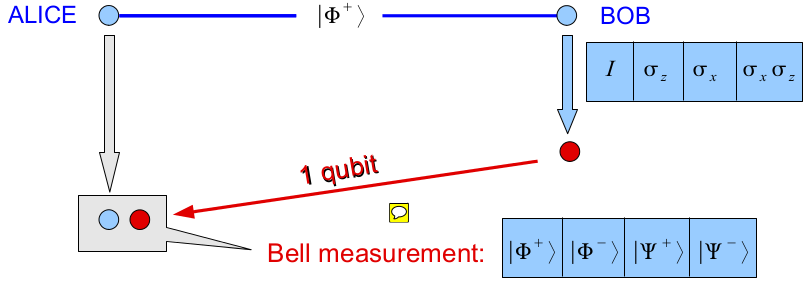
\includegraphics[scale=0.25]{ch2/image6}
	\captionof{figure}{ }
	\end{wrapfigure}
Supposons qu'Alice et Bob se partagent un état $\ket{\Phi^+}$, mais ils ne peuvent
communiquer avec lui. Bob applique une des quatre opérations possible ($I, \sigma_z, 
\sigma_x,\sigma_x\sigma_z$). Ce qui l'intéresse c'est transmettre deux bits (soit 
quatre possibilités).\\

Le qbit d'Alice ne change pas, elle ne peut pas savoir ce qui se passe du côté de Bob,
mais Bob envoie son qbit à Alice. Une fois qu'Alice le reçoit, elle est en possession
de deux qbits et peut faire une \textbf{mesure de Bell}\footnote{Mesure qui nous dit dans
lequel des quatre états de Bell on se trouve.}. Alice sait ce qu'elle a, partage
un état intriqué avec Bob et la mesure de Bell lui donne un des quatre états de \textsc{Bell} 
possibles
\begin{equation}
\ket{\Phi^+},\qquad\ket{\Phi^-},\qquad\ket{\Psi^+},\qquad\ket{\Psi^-}
\end{equation}
Elle est donc en mesure de savoir ce qu'a appliqué Bob sur l'état de \textsc{Bell} partagé. 
L'information de ce qu'a appliqué Bob tenant dans deux bits, nous avons bien transféré deux
bits à l'aide d'un seul qbit à l'aide de l'intrication. On ne peut donc pas transmettre 
d'information via cet état, mais on peut l'utiliser pour faire du codage dense. La causalité
n'a ici pas été violée car Bob a du envoyer son qbit à Alice via un système physique, 
causal\footnote{Voir slide 44 (cours1) sur les EPR. Je n'ai pas de notes dessus.}.


\subsection{Téléportation quantique}
Alice reçoit un qbit $\ket{\Psi} = \alpha\ket0+\beta\ket1$ et partage un état de \textsc{Bell}
$\ket{\Phi^+} = \frac{1}{\sqrt{2}}\left(\ket{00}+\ket{11}\right)$ avec Bob.
\begin{center}
	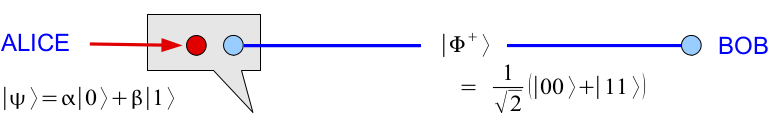
\includegraphics[scale=0.4]{ch2/image7}
	\captionof{figure}{ }
\end{center}

\newpage
 Faisons le produit
des deux états d'Alice (à gauche le qbit que l'on souhaite téléporter, à droite l'intriqué)
\begin{equation}
\begin{array}{ll}
\ket{\Psi}\ket{\Phi^+} &\DS= \frac{1}{\sqrt{2}}\left(\ket{00}+\ket{11}\right)\left(
\alpha\ket0+\beta\ket1\right)\\
&=\DS \frac{1}{\sqrt{2}}\left( \alpha\underbrace{\ket{00}}_{\frac{\Phi^++\Phi^-}{\sqrt{2}}}\ket0
+\alpha\underbrace{\ket{01}}_{\frac{\Psi^++\Psi^-}{\sqrt{2}}}\ket1+
\beta\underbrace{\ket{10}}_{\frac{\Psi^+-\Psi^-}{\sqrt{2}}}\ket0+\beta\underbrace{\ket{11}}_{\frac{\Phi^+-\Phi^-}{\sqrt{2}}}\ket1
\right)
\end{array}
\end{equation}
Il est important de remarquer ici que le premier produit correspond à 
\begin{equation}
\frac{\alpha}{\sqrt{2}}\ket{00}_{AC}\ket{0}_B
\end{equation}
où $C$ désigne le qbit à téléporter. Les qbits $\ket{..}$ correspondent à $AC$ (les deux 
qubits de $A$) tandis que les $\ket{.}$ correspondent aux qubit que $B$ à en sa possession !
On peut regrouper les termes en $\Phi^+$ ce qui fait apparaître $\ket\Psi =(\alpha\ket{0}_B+
\beta\ket{1}_B)$, l'état à 
téléporter. En faisant de même pour les autres états de \textsc{Bell}
\begin{equation}
\ket{\Psi}\ket{\Phi^+} = \frac{1}{2}\left(\ket{\Phi^+}\underbrace{\left(\alpha\ket0+\beta\ket1
\right)}_{\ket\Psi}+\ket{\Phi^-}\underbrace{\left(\alpha\ket0-\beta\ket1
\right)}_{\sigma_z\ket\Psi}\right)
+
\frac{1}{2}\left(\ket{\Psi^+}\underbrace{\left(\alpha\ket1+\beta\ket0
\right)}_{\sigma_x\ket\Psi}+\ket{\Psi^-}\underbrace{\left(\alpha\ket1-\beta\ket0
\right)}_{\sigma_x\sigma_z\ket\Psi}\right)
\end{equation}
Nous voyons apparaître dans l'ordre le qbit à téléporter, le qbit à téléporter avec un 
\textit{SIGN-FLIP}, toujours le même avec un \textit{BIT-FLIP} et enfin la combinaison
des deux. Nous avons ici juste ré-écrit l'état original. Réécrivons-le
\begin{equation}
\ket\Psi\ket{\Phi^+} = \frac{1}{2}\left(\ket{\Phi^+}\ket{\Psi}+
\ket{\Phi^-}\sigma_z\ket{\Psi}+\ket{\Psi^+}\sigma_x\ket{\Psi}+\ket{\Phi^-}\sigma_x\sigma_z\ket{\Psi}
\right)
\end{equation}
Alice va faire une \textbf{mesure de Bell} sur les \textbf{deux} qbits qu'elle possède (celui à 
téléporter et l'intriqué) : c'est la que va véritablement se faire la téléportation. En effet, en
effectuant la mesure, le résultat d'Alice est que l'état à trois particules va se réduire à l'un
des quatre états suivant (probabilité identique)
\begin{equation}
\ket{\Phi^+}\ket{\Psi},\qquad\qquad
\ket{\Phi^-}\sigma_z\ket{\Psi},\qquad\qquad\ket{\Psi^+}\sigma_x\ket{\Psi},\qquad\qquad\ket{\Phi^-}\sigma_x\sigma_z\ket{\Psi}
\label{eq:cc}
\end{equation}
Les qbits d'Alice sont maintenant intriqués dans l'un des quatre états de Bell\footnote{Lorsque 
l'on fait une mesure de Bell sur des états qui n'étaient pas de Bell avant, ils sont projeter sur un état de Bell et ils deviennent intriqués.} et l'intrication initialement partagée par Alice et Bob est cassée :
le qbit de Bob est dans un des états \eqref{eq:cc}.\footnote{Ca ne viole pas la causalité ? C'est bien le principe de réduction de la fonction d'onde? Un peu étrange. En fait, non : les qbits de Psi dans 2.31 sont ceux de Bob ! Voir page eng Wiki ou c'est explicité (ou ce que j'ai rajouté). C'est juste que les psi et psi modifié par les matrices sont le qbit de bob : on se réduit à une des fonctions et pour retrouver le bit (bob a un bit modifié) il doit appliquer la transfo que lui dit alice} Le qbit de Bob ressemble maintenant à celui qui doit être téléporté, mais il n'est le même que dans $1/4$ des cas.\\

Lorsque Alice a effectué la mesure de Bell sur ses qbits, elle a mesuré l'état de Bell dans lequel
elle se trouve. Par exemple, si Alice a mesuré $\ket{\Psi^+}$, elle sait que l'on a appliqué $\sigma_x$ sur $\ket\Psi$. Il y a quatre mesures possibles, qui correspondent à quatre opérations distinctes faite sur $\ket\Psi$
\begin{equation}
I,\qquad\qquad \sigma_z,\qquad\qquad\sigma_x,\qquad\qquad\sigma_x\sigma_z
\end{equation}
Ces opérations se codent en deux bits. Alice va envoyer ces deux bits à Bob ce qui permettra de 
savoir à Bob "ce qu'il a entre les mains" et de retrouver exactement $\ket\Psi$ (et pas quelque
chose qui "lui ressemble", comme dans $3/4$ des cas). Quelques exemples :

\begin{itemize}
\item[$\bullet$] Si Alice dit '00', Bob est en $\ket\Psi$ : il doit appliquer $I$, soit ne rien faire. 
\item[$\bullet$] Si Alice mesure $\ket{\Phi^-}$, elle envoie '01' ce qui correspond aux second
terme. Bob sait que l'état téléporté (qu'il "a entre les mains) à eu un \textit{SIGN-FLIP} : il en réapplique un autre pour retrouver l'état à téléporter. 
\end{itemize}

Alice envoie donc deux bits, Bob applique une transformation et grâce à ça il le "re-matérialise" 
sur une autre particule.\\

Remarques :
\begin{itemize}
\item Ca ne viole pas le principe du non-clonage car le qbit d'Alice est détruit
\item Le qbit de Bob ne contient pas d'information (pas causalement lié à celui d'Alice)
\item Les bits transmis classiquement ne cotiennent pas d'information (sinon le qubit serait
perturbé)
\end{itemize}

La section "Performing a Bell measurement using a BS" a été passée. Il reste la démonstration
expérimentale au slide 53, mais comme c'est l'article que j'ai choisi je ne détaille pas ici.



\iffalse


\fi